% Owner: Sharjeel Shahid 24L-3055
\section{Error Analysis and Bias}
\label{sec:error-bias}

There are no demographic subgroups in these market data. The relevant subgroups instead describe market conditions: the true direction class, volatility regime, outlier status, calendar year and named events. Class groups follow the true up/down label, outlier groups follow the saved \texttt{is\_outlier} flag, and calendar groups follow the prediction date. Volatility groups use tercile cuts fitted once to unique training dates, then apply those same cuts to every model and split. Event windows cover March--April 2020 for COVID in training, calendar year 2022 for rate rises in validation, and calendar year 2026 for the surge in testing. These names identify periods, not estimated causal effects.

The five models, \texttt{majority}, \texttt{logreg}, \texttt{random\_forest}, \texttt{hist\_gb} and \texttt{lstm}, are evaluated on the same 502 validation dates and 701 test dates. The LSTM has fewer training predictions because its first complete window requires earlier context, so training comparisons use the rows actually available for each model. All results below come from the saved segment and bias tables. Decimal metrics follow the truncation convention in Section~\ref{sec:deep}.

\subsection{Where the Models Fail}
% Sources: results/analysis/segment_metrics.csv class rows and bias_check.csv, split=test.
\begin{table}[H]
    \centering
    \small
    \begin{tabular}{lrrr}
        \toprule
        Model & Accuracy & Recall up & Recall down \\
        \midrule
        majority       & 0.6091 & 1.0000 & 0.0000 \\
        logreg         & 0.4978 & 0.3114 & 0.7883 \\
        random\_forest & 0.3908 & 0.0000 & 1.0000 \\
        hist\_gb       & 0.3908 & 0.0000 & 1.0000 \\
        lstm           & 0.5221 & 0.4847 & 0.5802 \\
        \bottomrule
    \end{tabular}
    \caption{Test-split accuracy and class recall. Accuracy alone hides complete failure on one direction class.}
    \label{tab:b-error-test}
\end{table}

\begin{figure}[H]
    \centering
    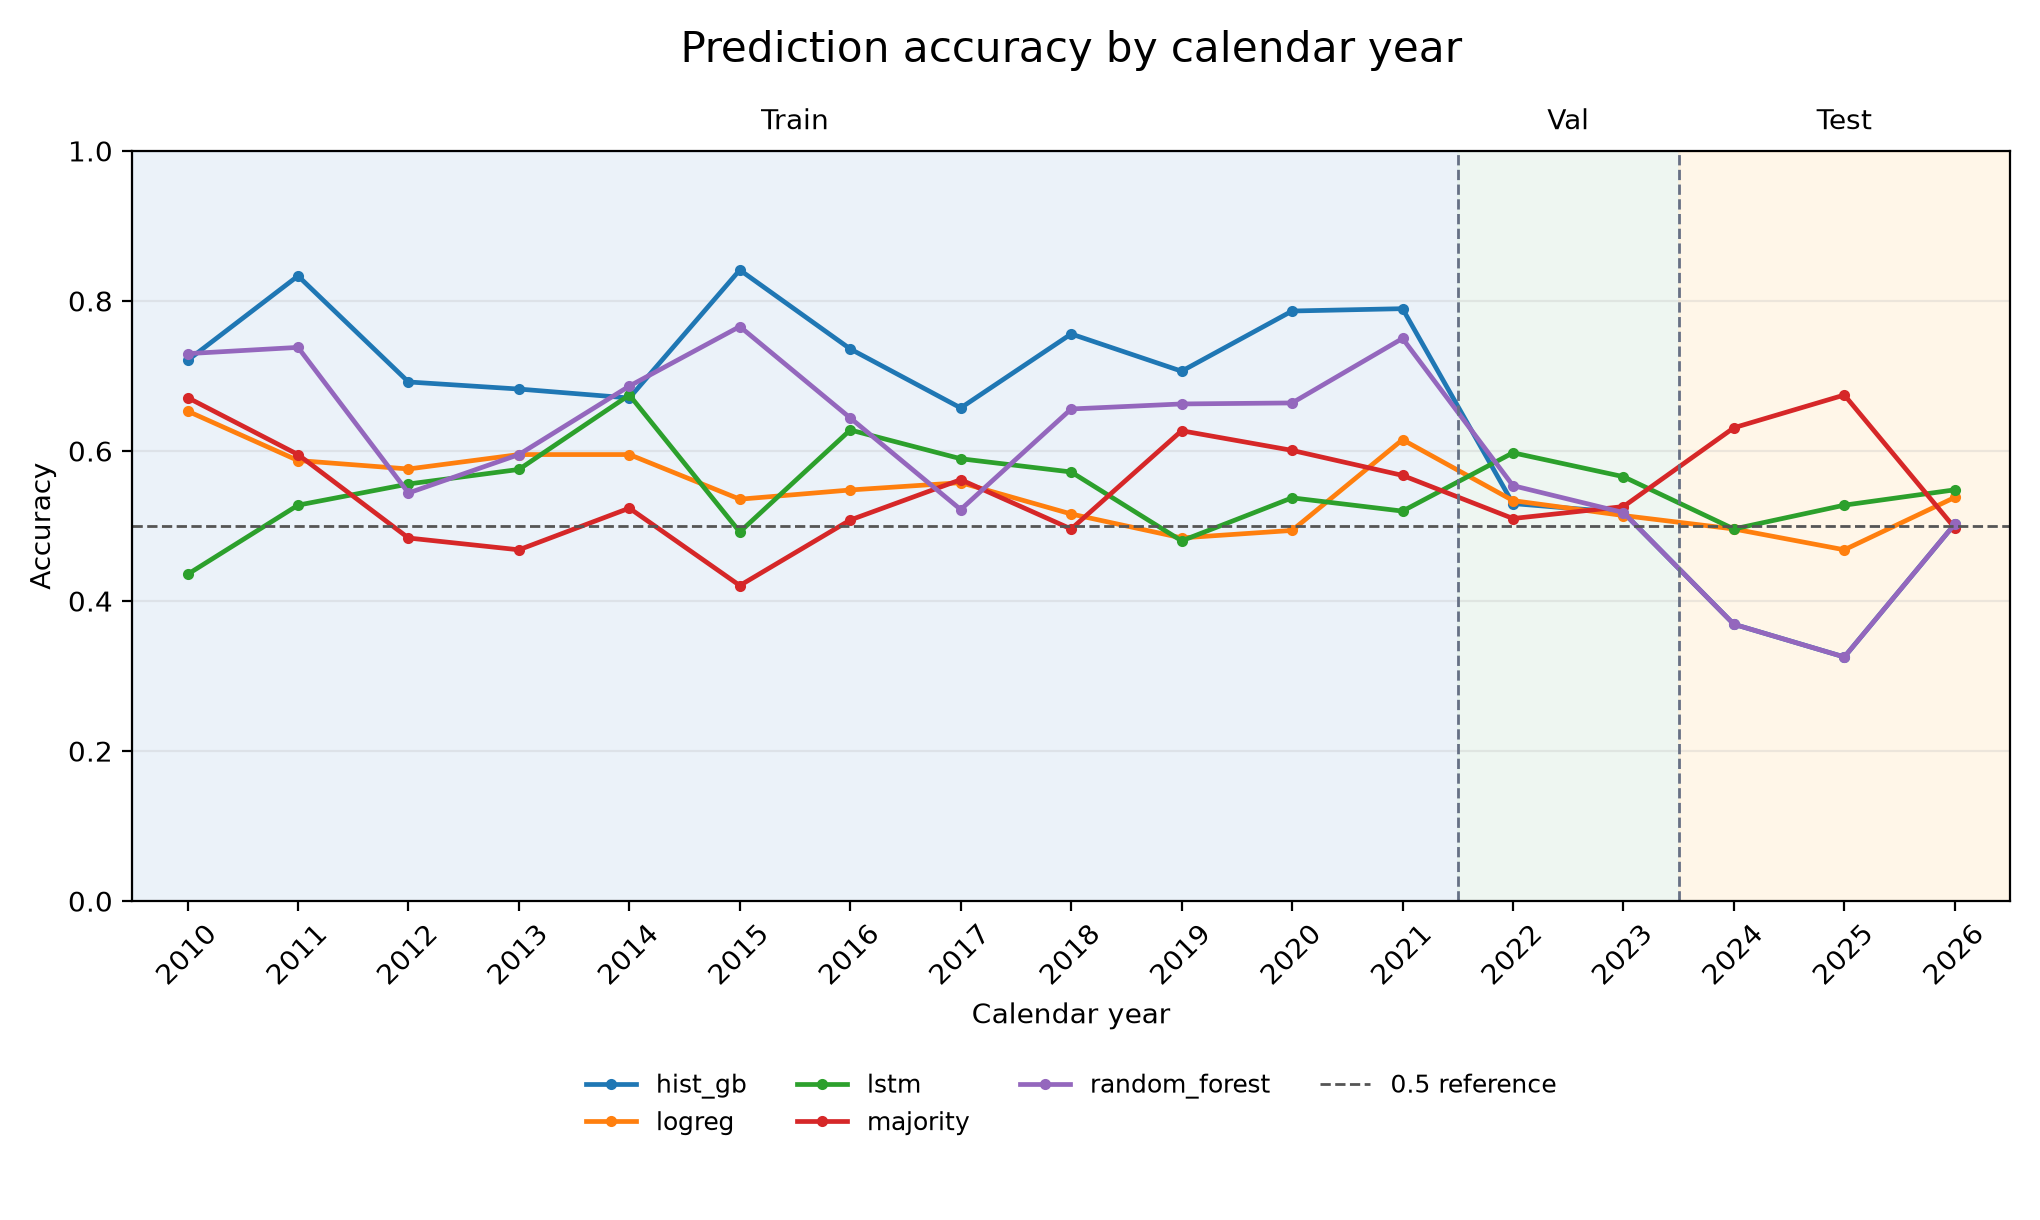
\includegraphics[width=0.95\textwidth]{analysis/accuracy_by_year.png}
    \caption{Accuracy by calendar year for all models. The split shading separates training, validation and testing; the horizontal dashed line marks 0.5. Training years are in-sample results.}
    \label{fig:b-error-year}
\end{figure}

% Source: segment_metrics.csv, segment_type=year, split=test.
\paragraph{Calendar years.}
The LSTM's test accuracy is 0.4960 in 2024 and 0.5277 in 2025, with 252 rows in each year. In 2026 it is 0.5482 on 197 rows, compared with 0.4974 for the majority model. Both tree models move from 0.3690 in 2024 and 0.3253 in 2025 to 0.5025 in 2026, while still predicting down on every test day. Their apparent improvement therefore reflects the changing class balance rather than recovered discrimination. Logistic regression reaches accuracy 0.5380 in 2026 but recalls only 0.0918 of the up cases in that year. The partial final year and the different class mixes limit direct comparisons across years.

\begin{figure}[H]
    \centering
    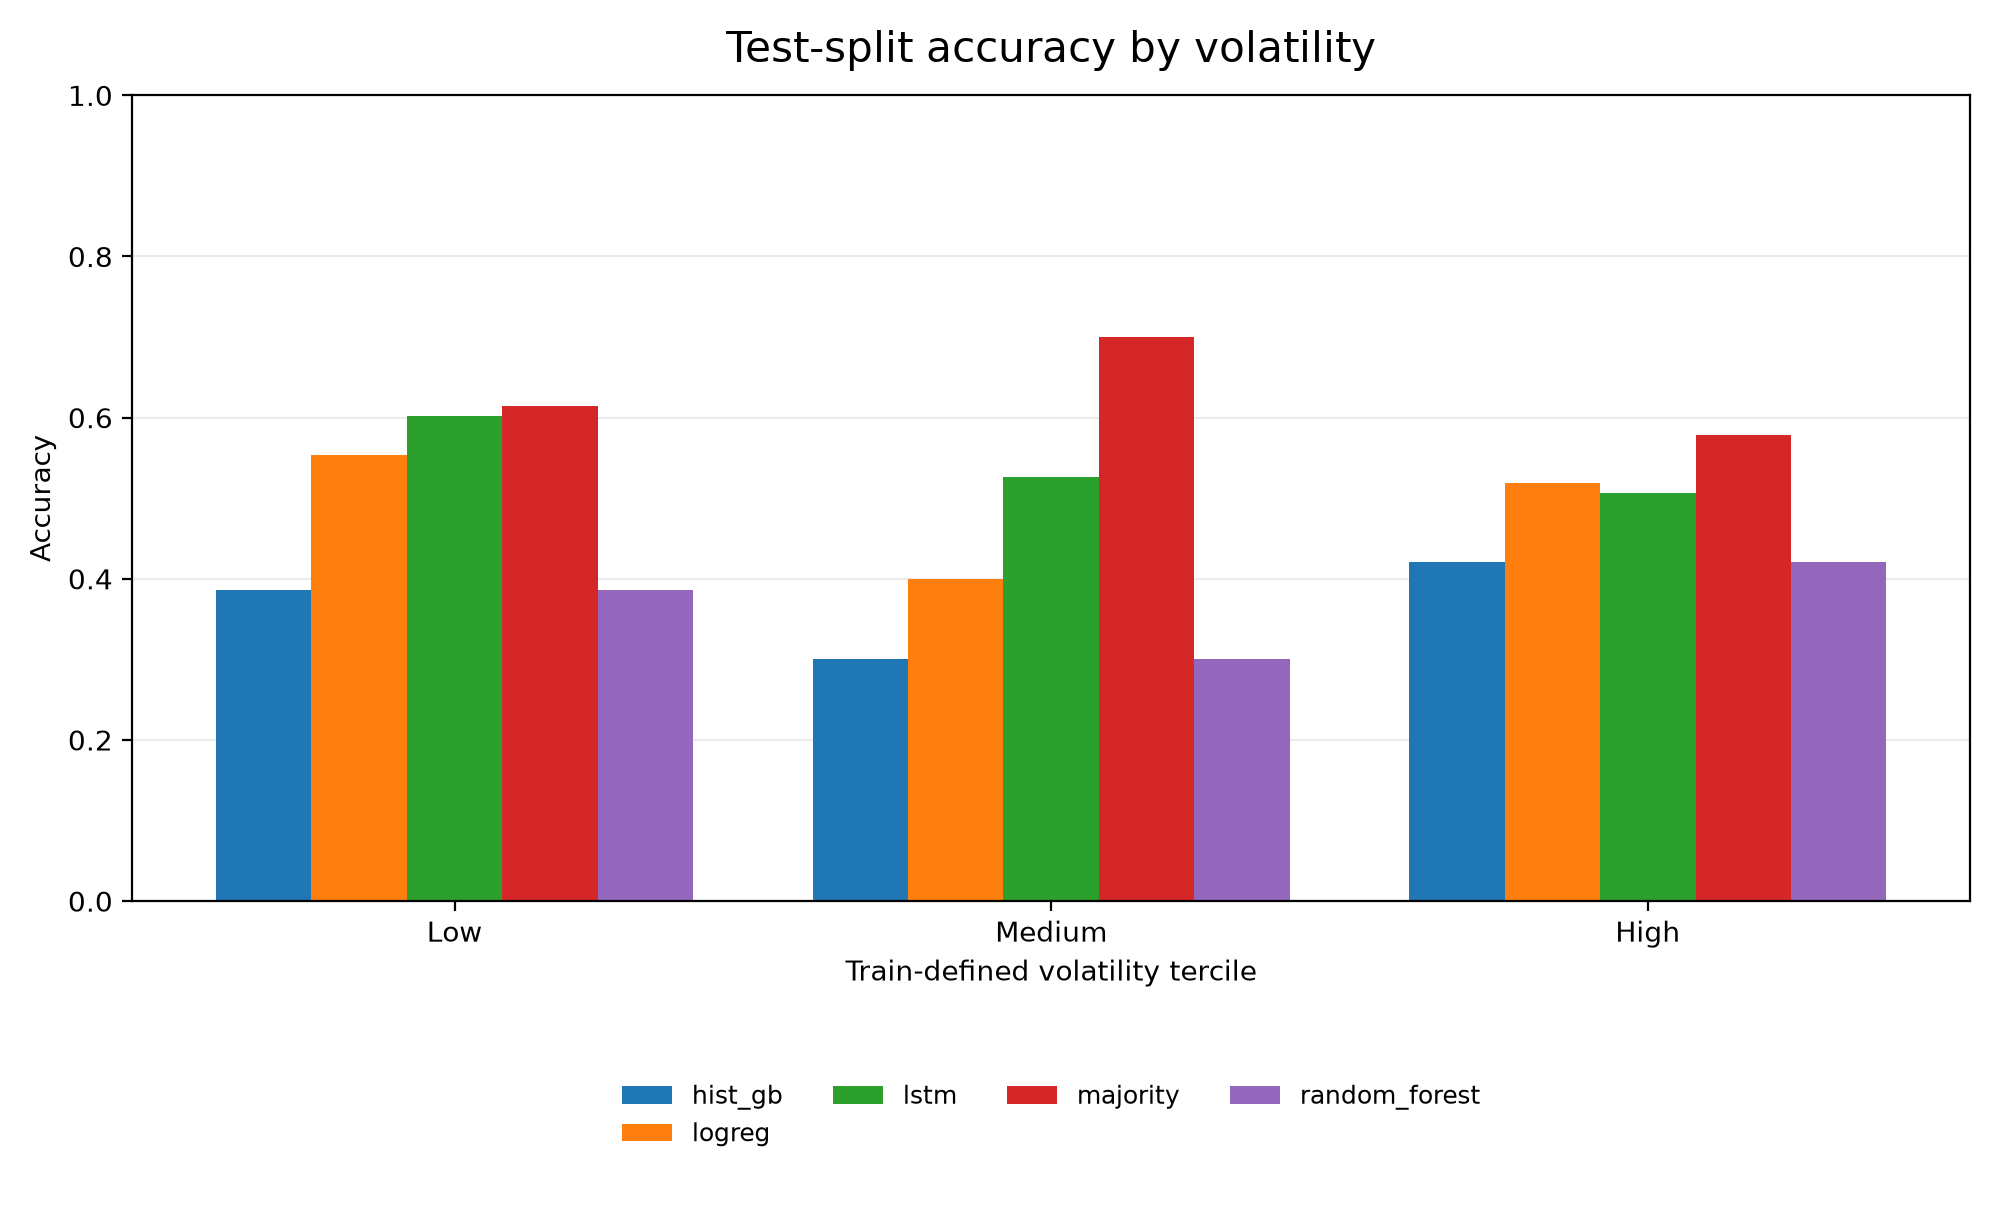
\includegraphics[width=0.90\textwidth]{analysis/accuracy_by_volatility.png}
    \caption{Test accuracy by volatility regime, using tercile thresholds fitted on training dates only. Test groups need not contain equal numbers of observations.}
    \label{fig:b-error-volatility}
\end{figure}

% Source: segment_metrics.csv, segment_type=volatility, split=test.
\paragraph{Volatility.}
The low-, medium- and high-volatility test groups contain 83, 150 and 468 rows. LSTM accuracy decreases across these groups from 0.6024 to 0.5266 to 0.5064. Logistic regression has accuracy 0.5192 in the high-volatility group, slightly above the LSTM there. The majority model has higher accuracy than every learned model within each volatility group. The low-volatility estimate is based on the smallest group and is correspondingly more uncertain; the row counts alone do not quantify that uncertainty.

% Source: segment_metrics.csv, segment_type=outlier, split=test.
\paragraph{Outlier days.}
There are 42 outlier rows and 659 normal rows in the test split. LSTM accuracy is 0.6190 on outliers and 0.5159 on normal days, compared with majority-model accuracies of 0.5952 and 0.6100. The apparent advantage on outliers is based on a small segment and is not evidence of a reliable advantage on rare events.

% Source: segment_metrics.csv, segment_type=event.
\paragraph{Named events.}
The COVID training window has only 43 rows per model. The LSTM has accuracy 0.5813, up recall 1.0000 and down recall 0.0526 in that window; \texttt{hist\_gb} has accuracy 0.7674. These are in-sample results, not an independent crisis test. The 2022 rate-rise validation segment contains 251 rows, on which the LSTM's accuracy of 0.5976 is the highest among the saved models, but this period also contributed to model selection. The 2026 surge event contains the same 197 test rows as the calendar-year segment, with LSTM accuracy 0.5482; it supplies no additional independent evidence.

\begin{figure}[H]
    \centering
    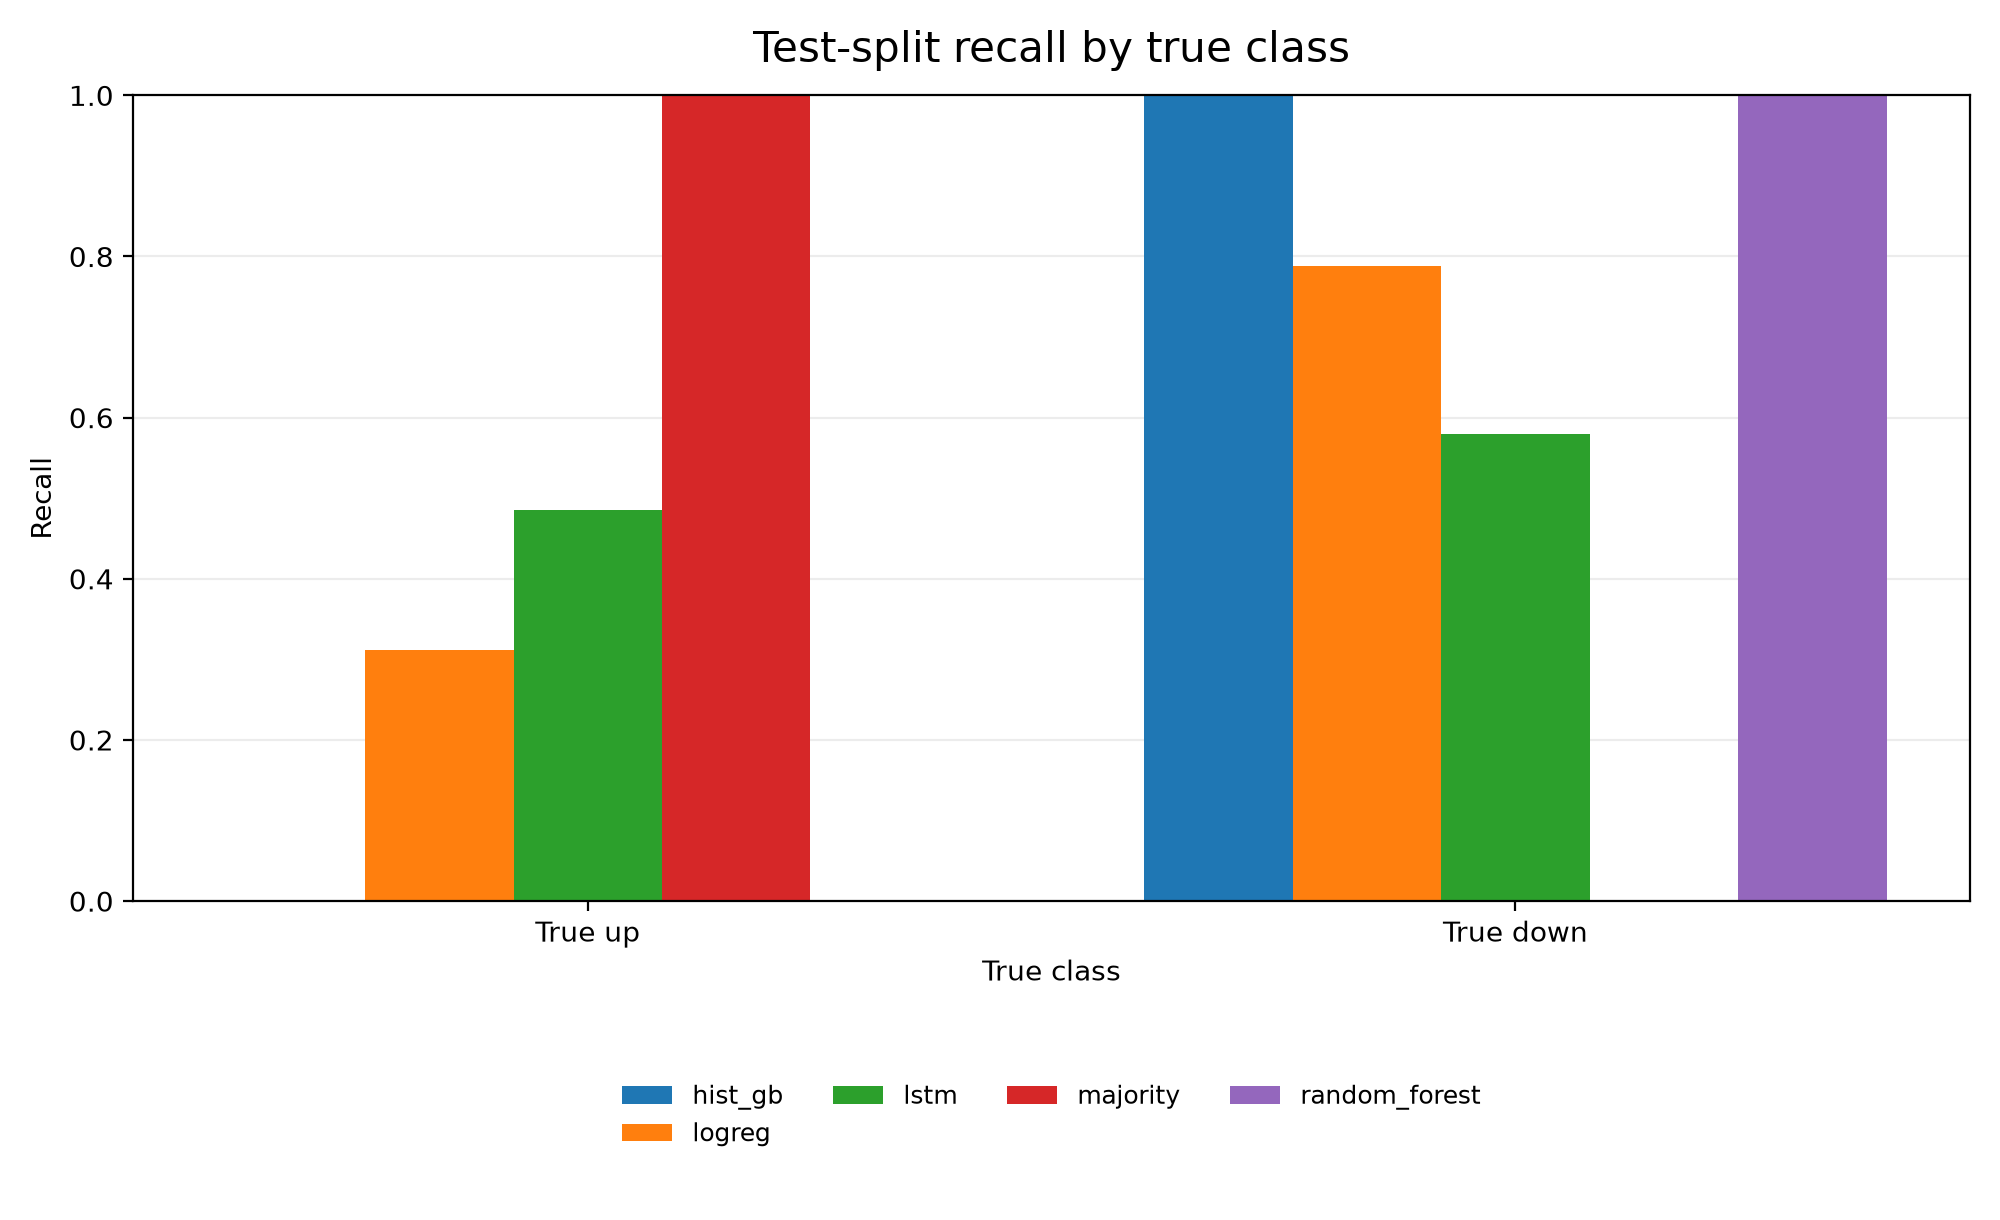
\includegraphics[width=0.90\textwidth]{analysis/recall_by_class.png}
    \caption{Test recall for up and down labels. A zero-height bar indicates zero recall for that class, rather than a missing model.}
    \label{fig:b-error-recall}
\end{figure}

Consecutive five-day-ahead labels overlap in their future-price intervals, so the effective sample size is smaller than the row count. Small event and outlier segments are particularly noisy. Confidence intervals and statistical significance were not measured for these comparisons.

\subsection{Bias Check}
Here bias means a directional prediction imbalance rather than demographic unfairness. The gap is predicted up-rate minus true up-rate. The baseline predicts each model's own training-majority class on every split, rather than choosing the majority class from test labels. That training-majority class is up for every model in the saved data.

% Source: results/analysis/bias_check.csv, split=test; all rate columns shown without percentages.
\begin{table}[H]
    \centering
    \small
    \begin{tabular}{lrrrrr}
        \toprule
        Model & \shortstack{True up\\rate} & \shortstack{Pred. up\\rate} & Gap & \shortstack{Majority\\accuracy} & \shortstack{Model\\accuracy} \\
        \midrule
        majority       & 0.6091 & 1.0000 &  0.3908 & 0.6091 & 0.6091 \\
        logreg         & 0.6091 & 0.2724 & -0.3366 & 0.6091 & 0.4978 \\
        random\_forest & 0.6091 & 0.0000 & -0.6091 & 0.6091 & 0.3908 \\
        hist\_gb       & 0.6091 & 0.0000 & -0.6091 & 0.6091 & 0.3908 \\
        lstm           & 0.6091 & 0.4593 & -0.1497 & 0.6091 & 0.5221 \\
        \bottomrule
    \end{tabular}
    \caption{Test-split directional bias and accuracy against the training-majority baseline. The gap is computed from the untruncated rates before display.}
    \label{tab:b-bias-test}
\end{table}

\paragraph{Class collapse.}
Both \texttt{random\_forest} and \texttt{hist\_gb} predict down on every test day: up recall is zero and down recall is one. The \texttt{majority} model always predicts up and has the opposite recall pattern. All three therefore meet the analysis flag ``COLLAPSED to one class'', although constant prediction is intentional for the baseline. Logistic regression and the LSTM predict both classes, but both underpredict up relative to its observed frequency.

% Sources: bias_check.csv train/test true_up_rate; features_test.csv gold mean; classical_tuning.csv feature-set comparisons.
\paragraph{Distribution shift.}
The true up-rate changes from 54.25\% on the classical models' training rows to 60.91\% on test. The corresponding LSTM training rate is 53.97\%, reflecting its shorter training prediction coverage. The 2024--2026 gold price-level distribution is also shifted far from training: the mean scaled test gold value is 8.3554 training standard deviations above the training mean. This shift is a plausible mechanism consistent with the collapse of the level-based tree models and the absence of complete collapse in the stationary-feature LSTM. It is not a causal explanation established by these experiments: the models differ in architecture, training and feature selection. Moreover, Hassan's classical tuning table shows that the best stationary-feature variant of each learned classical model did not beat its best all-feature variant on the recorded cross-validation score. Simply replacing all price levels is therefore a proposal for further testing, not an improvement demonstrated by these results.

\paragraph{Comparison with the baseline.}
None of the learned models beats always-up test accuracy, which is 0.6091; the majority model matches it by construction. The LSTM has the highest accuracy among the learned models at 0.5221 and the smallest absolute directional-rate gap among them at 0.1497. It is therefore the least biased learned model by this particular aggregate measure, while still failing to beat the baseline on accuracy. This does not establish general fairness or reliable performance in every regime: its high-volatility and normal-day results remain weak, and the more favourable outlier result has limited support.

\paragraph{Changes to evaluate next.}
The following are proposals, not measured improvements:
\begin{itemize}
    \item Compare stationary and return-based feature sets across all model families, with past-only rolling or expanding re-scaling to reduce sensitivity to changing price levels.
    \item Use walk-forward refits as new data arrive and purge forward-looking labels consistently at validation boundaries.
    \item Tune decision thresholds or calibrate probabilities on validation data, then assess the fixed choices on untouched future periods.
    \item Repeat with multiple seeds, dependence-aware confidence intervals, and a longer or complete tuning grid.
    \item Assess AUC and balanced accuracy alongside ordinary accuracy, and evaluate transaction costs and trading utility separately before drawing investment conclusions.
\end{itemize}

\paragraph{Limitations.}
The LSTM evidence comes from a single seed, a partial grid, and one validation period used for both checkpoint selection and configuration selection. Its unpurged validation boundary can include forward-label prices from the test calendar period. Overlapping labels and small segments reduce the amount of independent evidence. Transaction costs and trading profitability were not evaluated. These predictive comparisons are not financial advice.
